\documentclass[research]{BMSTU-IU8}

\usepackage{fontspec}
\setmainfont{Times New Roman}
\setromanfont{Times New Roman} 
\setsansfont{Arial} 
\setmonofont{Courier New}

\usepackage{todonotes}
\usepackage{lipsum}
\usepackage{tikz}
\usepackage{pgfplots}

\student{Санджиев Т. С.}
\theme{Подготовка датасета для обучения классификатора криптовалютных транзакций}
\group{ИУ8-93-2024}

\studentFullName{Санджиев Темирхан Санджиевич}
\profile{20У951}
\speciality{10.05.03 <<Информационная безопасность автоматизированных систем>>}
\specialization{10.05.03\_03 <<Создание автоматизированных систем в защищенном исполнении>>}
\supervisorWithDegree{профессор кафедры ИУ8 Зуев Юрий Анатольевич}
\supervisor{Зуев Ю. А.}

\addbibresource{main.bib}
% Сокращения и обозначения
\newacronym{sarif}{SARIF}{Static Analysis Results Interchange Format}
\newacronym{api}{API}{Application Programming Interface}
\newacronym{csv}{CSV}{Comma-Separated Values}
\newacronym{sql}{SQL}{Structured Query Language}
\newacronym{json}{JSON}{JavaScript Object Notation}
\newacronym{git}{Git}{Distributed Version Control System}
\newacronym{github}{GitHub}{Web-based Git repository hosting service}
\newacronym{postgresql}{PostgreSQL}{Object-relational database management system}
\newacronym{go}{Go}{Programming language developed by Google}
\newacronym{goroutine}{Goroutine}{Lightweight thread managed by Go runtime}
\newacronym{semaphore}{Semaphore}{Synchronization primitive for controlling access to resources}
\newacronym{ci}{CI}{Continuous Integration}
\newacronym{cd}{CD}{Continuous Deployment}
\newacronym{sast}{SAST}{Static Application Security Testing}
\newacronym{ast}{AST}{Abstract Syntax Tree}
\newacronym{cpu}{CPU}{Central Processing Unit}
\newacronym{ram}{RAM}{Random Access Memory}
\newacronym{io}{I/O}{Input/Output}
\newacronym{url}{URL}{Uniform Resource Locator}
\newacronym{http}{HTTP}{Hypertext Transfer Protocol}
\newacronym{https}{HTTPS}{HTTP Secure}

% Термины и определения
\newglossaryentry{id1}{
    name={Bitcoin},
    description={Криптовалюта и одноименная платежная система, использующая одноименную единицу для учета операций}
}

\newglossaryentry{id2}{
    name={Блокчейн},
    description={Распределенная база данных, состоящая из последовательно связанных блоков, содержащих информацию о транзакциях}
}

\newglossaryentry{id3}{
    name={Транзакция},
    description={Операция передачи Bitcoin между адресами, записанная в блокчейне}
}

\newglossaryentry{id4}{
    name={Адрес},
    description={Уникальный идентификатор в сети Bitcoin, используемый для отправки и получения средств}
}

\newglossaryentry{id5}{
    name={UTXO},
    description={Unspent Transaction Output - модель учета средств в Bitcoin, где каждый выход транзакции может быть потрачен только один раз}
}

\newglossaryentry{id6}{
    name={Кошелек},
    description={Программное обеспечение или устройство для хранения, отправки и получения Bitcoin}
}

\newglossaryentry{id7}{
    name={Майнинг},
    description={Процесс создания новых блоков в блокчейне Bitcoin путем решения криптографических задач}
}

\newglossaryentry{id8}{
    name={Хеш},
    description={Результат применения криптографической хеш-функции к данным, используется для обеспечения целостности и безопасности}
}

\newglossaryentry{id9}{
    name={Приватный ключ},
    description={Секретный ключ, используемый для подписи транзакций и доступа к средствам на Bitcoin-адресе}
}

\newglossaryentry{id10}{
    name={Публичный ключ},
    description={Криптографический ключ, доступный всем участникам сети, используется для проверки подписей транзакций}
}

\newglossaryentry{id11}{
    name={Блок},
    description={Структура данных, содержащая набор транзакций и метаданные, является частью блокчейна}
}

\newglossaryentry{id12}{
    name={Узел},
    description={Компьютер в сети Bitcoin, который поддерживает копию блокчейна и участвует в валидации транзакций}
}

\newglossaryentry{id13}{
    name={Консенсус},
    description={Механизм достижения согласия между узлами сети о состоянии блокчейна}
}

\newglossaryentry{id14}{
    name={Proof of Work},
    description={Алгоритм консенсуса, требующий от майнеров решения вычислительно сложных задач для создания блоков}
}

\newglossaryentry{id15}{
    name={Дерево Меркла},
    description={Структура данных, используемая для эффективной проверки целостности большого количества транзакций в блоке}
}

\newglossaryentry{id16}{
    name={Script},
    description={Язык программирования Bitcoin, используемый для определения условий траты средств}
}

\newglossaryentry{id17}{
    name={Мультиподпись},
    description={Механизм, требующий подписи нескольких приватных ключей для выполнения транзакции}
}

\newglossaryentry{id18}{
    name={SegWit},
    description={Segregated Witness - обновление протокола Bitcoin, отделяющее данные подписей от данных транзакций}
}

\newglossaryentry{id19}{
    name={Lightning Network},
    description={Протокол второго уровня для Bitcoin, обеспечивающий быстрые и дешевые микроплатежи}
}

\newglossaryentry{id20}{
    name={CoinJoin},
    description={Метод повышения приватности в Bitcoin, объединяющий входы и выходы нескольких пользователей в одну транзакцию}
}

\newglossaryentry{id21}{
    name={Coinbase транзакция},
    description={Специальная транзакция, создаваемая майнером в каждом блоке для получения вознаграждения за майнинг}
}

\newglossaryentry{id22}{
    name={Извлечение признаков},
    description={Процесс выделения характеристик из данных для использования в алгоритмах машинного обучения}
}

\newglossaryentry{id23}{
    name={Классификация},
    description={Задача машинного обучения, заключающаяся в отнесении объектов к предопределенным классам}
}

\newglossaryentry{id24}{
    name={Датасет},
    description={Набор данных, используемый для обучения, тестирования и валидации алгоритмов машинного обучения}
}

\newglossaryentry{id25}{
    name={API клиент},
    description={Программный компонент, обеспечивающий взаимодействие с внешним API для получения данных}
}

\newglossaryentry{id26}{
    name={Ограничение скорости},
    description={Механизм контроля частоты запросов к API для предотвращения перегрузки сервера}
}

\newglossaryentry{id27}{
    name={Параллельная обработка},
    description={Метод выполнения вычислений одновременно на нескольких процессорах или потоках}
}

\newglossaryentry{id28}{
    name={Персистентность данных},
    description={Способность данных сохраняться после завершения работы программы}
}

\newglossaryentry{id29}{
    name={Инкрементальный сбор},
    description={Метод сбора данных, при котором обрабатываются только новые или измененные данные}
}


\begin{document}
    \maketitle
    
    \setcounter{page}{4}

    \abstract % Структурный элемент: РЕФЕРАТ
\textbf{Цель работы:} разработка комплексной методологии подготовки датасета для обучения классификатора типов Bitcoin-кошельков, включающей модули сбора данных через Bitcoin-эксплорер и извлечения признаков из транзакционных данных.

\textbf{Задачи исследования:} анализ существующих источников данных Bitcoin-адресов и их категоризации, разработка системы автоматизированного сбора данных через API Bitcoin-эксплорера, создание методологии извлечения 34 признаков из транзакционных данных, разработка алгоритмов анализа структурных, временных, экономических и сетевых паттернов, проведение комплексного статистического анализа извлеченных признаков, создание системы валидации и контроля качества данных.

\textbf{Объект исследования:} Bitcoin-адреса и связанные с ними транзакции в сети Bitcoin.

\textbf{Предмет исследования:} методы сбора, обработки и анализа данных о Bitcoin-адресах для создания качественных датасетов машинного обучения с целью классификации типов кошельков.

\textbf{Методы исследования:} анализ существующих датасетов Bitcoin-адресов, разработка алгоритмов сбора данных через REST API Bitcoin-эксплорера, методы извлечения признаков из транзакционных данных, статистический анализ качества данных, корреляционный анализ, методы машинного обучения для оценки важности признаков.

\textbf{Результаты:} разработана многоуровневая архитектура системы сбора данных с использованием API Bitcoin-эксплорера, создана методология извлечения 34 признаков, разделенных на 6 категорий (структурные, UTXO паттерны, временные, экономические, сетевые, поведенческие), проведен комплексный статистический анализ датасета из 8,115 Bitcoin-адресов с выявлением наиболее информативных признаков для классификации, создана система валидации и контроля качества данных с обработкой ошибок и параллельной обработкой.

\textbf{Практическая значимость:} результаты исследования могут быть использованы для создания качественных датасетов для обучения алгоритмов классификации типов Bitcoin-кошельков, автоматизации процессов подготовки данных для машинного обучения в области Bitcoin-аналитики, разработки инструментов для регуляторного надзора и анализа рисков в криптовалютных операциях, а также для исследования экономических паттернов в экосистеме Bitcoin.

\textbf{Ключевые слова:} Bitcoin, блокчейн, машинное обучение, классификация кошельков, датасет, извлечение признаков, Bitcoin-эксплорер, транзакционный анализ.

    \tableofcontents
    \termsanddefenitions
    \listofabbreviations
    
    \introduction % Структурный элемент: ВВЕДЕНИЕ

С момента появления Bitcoin в 2009 году эта криптовалюта стала неотъемлемой частью современной финансовой экосистемы. Децентрализованная природа Bitcoin, основанная на технологии блокчейн, обеспечивает прозрачность и безопасность транзакций, но одновременно создает возможности для злоупотреблений, таких как отмывание денег, мошенничество, фишинг и финансирование незаконной деятельности. В отличие от традиционных банковских систем, где информация о финансовых операциях доступна ограниченному кругу лиц, Bitcoin предоставляет открытый доступ к данным о транзакциях. Это делает его привлекательным для анализа, но также требует разработки эффективных алгоритмов классификации типов кошельков для выявления подозрительной активности в сети Bitcoin.

Классификация Bitcoin-адресов по типам кошельков является критически важной задачей в области анализа блокчейн-данных. Точная идентификация типов кошельков (биржи, майнеры, микшинг-сервисы, азартные игры) имеет практическое значение для регуляторного надзора, анализа рисков в криптовалютных операциях, исследования экономических паттернов в экосистеме Bitcoin и разработки инструментов для правоохранительных органов. Проблема классификации Bitcoin-адресов приобретает особую актуальность в связи с ростом объемов криптовалютных транзакций (ежедневный объем Bitcoin превышает 300,000 операций), регуляторными требованиями соблюдения AML/KYC процедур, необходимостью выявления подозрительной активности и мошеннических схем, а также исследовательскими задачами понимания экономических паттернов в криптовалютной экосистеме.

Ключевой проблемой в области анализа Bitcoin-транзакций является отсутствие качественных, сбалансированных и репрезентативных датасетов для обучения классификаторов типов кошельков. Существующие датасеты часто страдают от дисбаланса классов, неполноты данных и устаревших меток, что существенно ограничивает эффективность алгоритмов машинного обучения. Кроме того, быстрая эволюция сети Bitcoin и появление новых типов сервисов требуют постоянного обновления и расширения обучающих данных.

Целью данной научно-исследовательской работы является разработка комплексной методологии подготовки датасета для обучения классификатора типов Bitcoin-кошельков, включающей модули сбора данных через Bitcoin-эксплорер и извлечения признаков из транзакционных данных.

Основные задачи исследования:
\begin{itemize}
    \item Анализ существующих источников данных Bitcoin-адресов и их категоризации
    \item Разработка системы автоматизированного сбора данных через API Bitcoin-эксплорера
    \item Создание методологии извлечения 34 признаков из транзакционных данных
    \item Разработка алгоритмов анализа структурных, временных, экономических и сетевых паттернов
    \item Проведение комплексного статистического анализа извлеченных признаков
    \item Создание системы валидации и контроля качества данных
\end{itemize}

Актуальность работы обусловлена растущей потребностью в качественных датасетах для обучения алгоритмов классификации типов Bitcoin-кошельков, необходимостью автоматизации процессов подготовки данных для машинного обучения в области Bitcoin-аналитики, а также важностью понимания поведенческих паттернов различных типов участников криптовалютной экосистемы для регуляторного надзора и анализа рисков.

    \section{Модуль 1: Сбор данных для подготовки датасета по сети Bitcoin}
В рамках первого модуля НИРС была поставлена задача по сбору данных для подготовки датасета, предназначенного для обучения классификатора криптовалютных транзакций. Основной целью являлось создание структурированного набора данных, содержащего информацию об адресах Bitcoin и связанных с ними транзакциях.

Классификация Bitcoin-адресов по типам кошельков является критически важной задачей в области анализа блокчейн-данных. Точная идентификация типов кошельков (биржи, майнеры, микшинг-сервисы, азартные игры) имеет практическое значение для регуляторного надзора, анализа рисков в криптовалютных операциях, исследования экономических паттернов в экосистеме Bitcoin и разработки инструментов для правоохранительных органов.

Проблема классификации Bitcoin-адресов приобретает особую актуальность в связи с ростом объемов криптовалютных транзакций (ежедневный объем Bitcoin превышает 300,000 операций), регуляторными требованиями соблюдения AML/KYC процедур, необходимостью выявления подозрительной активности и мошеннических схем, а также исследовательскими задачами понимания экономических паттернов в криптовалютной экосистеме.

\subsection{Источники данных и методология сбора}

\subsubsection{Базовый источник данных}

В качестве базового источника данных был использован датасет Гарвардского университета \cite{harvard_dataset}. Данный датасет содержит пары "адрес-категория" для Bitcoin-адресов, где каждая категория представляет собой тип сервиса или организации, связанной с адресом. Датасет включает категории: exchange (биржи криптовалют), gambling (азартные игры), miner (майнеры), services (различные сервисы) и coinjoin-like (адреса, связанные с технологиями повышения приватности).

Для получения актуальных данных о Bitcoin-адресах и транзакциях был разработан автоматизированный процесс сбора данных через API Bitcoin-эксплорера \cite{bitcoin_explorer_api}\cite{walletexplorer_api}. Данный подход основан на принципах работы Bitcoin-сети, описанных в оригинальной работе \cite{bitcoin_whitepaper}, и использует методы анализа блокчейна, разработанные в исследованиях \cite{blockchain_analysis_survey, bitcoin_privacy_analysis, bitcoin_clustering}.

\textbf{Характеристики базового датасета.}
Базовый набор включает более 8{,}000 Bitcoin-адресов с верифицированными метками классов и охватывает период с 2009 по 2020 годы. Разметка выполнена на основе экспертной оценки, что обеспечивает высокое качество категорий, а данные регулярно актуализируются по мере появления новых транзакций. Использованы проверенные источники и процедуры валидации категорий, что позволяет опираться на датасет как на достоверную основу для последующего анализа.

\subsubsection{Архитектура системы сбора данных}

Для получения актуальных данных о Bitcoin-адресах и транзакциях была разработана многоуровневая архитектура системы сбора данных, основанная на принципах модульности, устойчивости и производительности. Архитектура представляет собой совокупность взаимосвязанных компонентов, каждый из которых отвечает за определенный аспект процесса сбора и обработки данных.

\textbf{Основные компоненты архитектуры системы:}

\textbf{CollectorConfig} представляет собой централизованную систему конфигурации, которая обеспечивает единообразное управление параметрами всей системы. Данный компонент включает настройки URL API-эндпоинтов, временные параметры (задержки между запросами, таймауты), параметры параллельной обработки (количество воркеров, размеры батчей), а также настройки retry-логики и контроля скорости запросов. Централизация конфигурации позволяет легко адаптировать систему под различные условия работы и требования API-провайдеров.

\textbf{Модели данных (AddressData/TransactionData)} обеспечивают структурированное представление адресов и транзакций Bitcoin. Эти модели включают типизированные поля для всех атрибутов адресов и транзакций, поддержку JSON сериализации для сложных структур данных, встроенную валидацию данных на уровне модели, а также механизмы обеспечения целостности данных. Использование строго типизированных моделей исключает ошибки, связанные с неправильным форматом данных, и обеспечивает консистентность на протяжении всего процесса обработки.

\textbf{WalletExplorerAPI} представляет собой специализированный HTTP-клиент, разработанный для взаимодействия с API Bitcoin-эксплорера \cite{walletexplorer_api}. Клиент реализует продвинутую retry-стратегию с экспоненциальным backoff для обработки временных сбоев, автоматическое управление rate limiting при получении HTTP 429 ошибок, настройку таймаутов и user-agent заголовков для имитации реального браузера, а также адаптивное управление задержками в зависимости от ответов сервера. Данный компонент обеспечивает надежное и эффективное взаимодействие с внешним API.

\textbf{DataPersistence} отвечает за управление персистентностью данных в системе. Компонент обеспечивает атомарные операции записи для предотвращения потери данных при сбоях, загрузку уже обработанных данных для реализации инкрементального сбора, использование CSV формата с JSON для сложных полей (inputs, outputs транзакций), а также восстановление состояния системы при перезапуске. Надежная система персистентности критически важна для долгосрочных процессов сбора данных.

\textbf{BitcoinDataCollector} является основным оркестратором всей системы, координирующим работу всех компонентов. Данный компонент реализует инкрементальную обработку данных с отслеживанием прогресса, параллельное выполнение операций с использованием ThreadPoolExecutor, управление жизненным циклом всех процессов, а также координацию между различными компонентами системы. Оркестратор обеспечивает целостность и эффективность всего процесса сбора данных.

\textbf{Принципы проектирования архитектуры:}

\textbf{Инкрементальность} является ключевым принципом архитектуры, обеспечивающим возможность продолжения сбора данных с места остановки. Система отслеживает все обработанные адреса и транзакции, пропускает уже собранные данные для минимизации дублирования запросов, автоматически восстанавливается после сбоев, и обеспечивает минимальные потери данных при прерывании процесса. Данный подход критически важен для долгосрочных проектов сбора данных, где полная перезагрузка может занять значительное время.

\textbf{Батчевая обработка} оптимизирует производительность системы через группировку операций. Адреса обрабатываются батчами по 20 записей, транзакции - батчами по 100 записей, что обеспечивает периодическое сохранение промежуточных результатов и минимизирует количество I/O операций. Батчевый подход также снижает нагрузку на API и улучшает общую производительность системы.

\textbf{Параллелизм} обеспечивает эффективное использование ресурсов системы. ThreadPoolExecutor используется для параллельной обработки адресов с настраиваемым количеством воркеров (по умолчанию 5), транзакции обрабатываются последовательно для избежания дублирования, а синхронизация доступа к общим ресурсам предотвращает конфликты. Параллельная обработка значительно ускоряет сбор данных при соблюдении лимитов API.

\textbf{Устойчивость} обеспечивает надежность системы в условиях нестабильной сети и внешних API. Система реализует retry с экспоненциальным backoff для обработки временных сбоев, специальную обработку HTTP ошибок (429, 5xx), graceful degradation при критических сбоях, а также комплексное логирование и мониторинг состояния системы. Устойчивость критически важна для долгосрочных процессов сбора данных, где сбои неизбежны.

\subsubsection{Детальная методология сбора}

\textbf{Детальная методология сбора данных:}

Методология сбора данных представляет собой комплексный процесс, состоящий из четырех основных этапов, каждый из которых имеет свои специфические задачи и механизмы реализации. Процесс начинается с инициализации системы, которая включает загрузку уже обработанных адресов и транзакций из CSV файлов для обеспечения инкрементальности, создание HTTP сессии с настроенной retry стратегией для обеспечения надежности соединений, настройку параметров параллелизма и батчинга в соответствии с возможностями системы и ограничениями API, а также инициализацию системы логирования для мониторинга процесса и отладки.

Сбор адресов представляет собой ключевой этап процесса, который начинается с фильтрации новых адресов путем исключения уже обработанных записей из базы данных. Затем система выполняет параллельные API вызовы с использованием ThreadPoolExecutor для максимального использования ресурсов системы, при этом соблюдая ограничения API по количеству одновременных запросов. Результаты сохраняются батчами каждые 20 адресов для минимизации потерь данных при сбоях, а список обработанных адресов обновляется в реальном времени для обеспечения инкрементальности процесса.

Сбор транзакций является следующим этапом, который включает извлечение уникальных идентификаторов транзакций (txid) из всех собранных адресов для избежания дублирования данных. Транзакции обрабатываются последовательно для предотвращения конфликтов и дублирования запросов, при этом каждая транзакция обогащается детальной информацией о входах, выходах, размере, времени и других атрибутах. Результаты сохраняются батчами каждые 100 транзакций для оптимизации производительности и минимизации нагрузки на файловую систему.

Система персистентности обеспечивает надежное хранение данных через атомарные операции записи в CSV файлы, что предотвращает потерю данных при сбоях системы. Сложные поля, такие как inputs и outputs транзакций, сериализуются в JSON формат для сохранения структурированности данных. Система обеспечивает восстановление состояния при перезапуске, что позволяет продолжить процесс сбора с места остановки, а также создает резервные копии критически важных данных для обеспечения долгосрочной надежности.

\textbf{Конфигурация системы} включает следующие ключевые параметры: задержка между запросами составляет 1.0 секунду для соблюдения лимитов API, количество параллельных воркеров установлено в 5 для оптимального баланса производительности и нагрузки на API, размер батча для адресов составляет 20 записей для эффективной обработки, размер батча для транзакций равен 100 записям для оптимизации I/O операций, таймаут HTTP запросов установлен в 30 секунд для обработки медленных соединений, количество повторов при ошибках составляет 3 для обеспечения надежности, а коэффициент экспоненциального backoff равен 0.3 для оптимального управления задержками при повторных попытках.

\subsubsection{Технические аспекты реализации}

\textbf{Технические аспекты реализации системы:}

Система обработки ошибок представляет собой многоуровневую архитектуру, обеспечивающую надежность работы в условиях нестабильной сети и внешних API. HTTP ошибки обрабатываются через retry механизм с экспоненциальным backoff, который автоматически увеличивает задержки между повторными попытками для снижения нагрузки на сервер. Rate limiting обрабатывается через автоматическое увеличение задержки при получении HTTP 429 ошибок, что позволяет системе адаптироваться к ограничениям API в реальном времени. Сетевые ошибки логируются с подробной информацией для последующего анализа, при этом система продолжает обработку других запросов. Некорректные данные валидируются с использованием fallback значений для обеспечения целостности датасета, а система восстановления обеспечивает автоматическое продолжение процесса сбора с места остановки при перезапуске.

Производительность системы оптимизирована через комплексный подход к управлению ресурсами. Параллелизм ограничен 5 одновременными запросами к API для соблюдения лимитов провайдера и предотвращения блокировки. Батчинг минимизирует I/O операции через группировку записей, что снижает нагрузку на файловую систему и улучшает общую производительность. Кэширование реализовано через отслеживание обработанных данных, что исключает дублирование запросов и оптимизирует использование ресурсов. Система автоматически пропускает уже обработанные адреса и транзакции, что обеспечивает эффективность инкрементального сбора данных.

Rate Limiting управляется через адаптивные механизмы, которые автоматически корректируют параметры системы в зависимости от ответов API. Адаптивные задержки увеличиваются при получении 429 ошибок и постепенно уменьшаются при успешных запросах, что обеспечивает оптимальный баланс между скоростью сбора и соблюдением ограничений API. User-Agent ротация использует различные заголовки для имитации различных браузеров и обхода ограничений, основанных на идентификации клиента. Мониторинг отслеживает статус API в реальном времени и автоматически корректирует параметры системы для обеспечения стабильной работы. Приоритизация обеспечивает обработку критически важных данных в первую очередь, что минимизирует потери при сбоях системы.

\subsubsection{Методология обработки и структурирования данных}

Методология обработки и структурирования данных в рамках первого модуля НИРС направлена на подготовку сырых данных для последующего анализа и извлечения признаков. Данная методология включает процессы очистки, нормализации, валидации и структурирования собранных данных о Bitcoin-адресах и транзакциях.

\textbf{Очистка данных:}

Процесс очистки данных начинается с удаления некорректных записей и дубликатов из собранного датасета. Система фильтрует неполные транзакции с отсутствующими входными или выходными данными, что критически важно для обеспечения целостности анализа. Проверка валидности Bitcoin-адресов выполняется с использованием криптографических алгоритмов для исключения некорректных записей. Дополнительно удаляются транзакции с нулевыми суммами или некорректными значениями, которые могут исказить результаты анализа.

\textbf{Нормализация данных:}

Нормализация обеспечивает единообразие представления данных для последующей обработки. Данные приводятся к единому формату с стандартизацией типов данных для всех полей. Временные метки стандартизируются путем приведения к UTC и использованию единого формата для всех временных характеристик. Единицы измерения унифицируются с использованием сатоши для сумм и байтов для размеров транзакций. Адреса нормализуются к стандартному формату Base58 для обеспечения консистентности.

\textbf{Валидация данных:}

Система валидации обеспечивает проверку целостности и корректности обработанных данных. Выполняется верификация балансов и сумм транзакций для выявления аномалий в данных. Контролируется соответствие меток классов исходным данным для обеспечения качества разметки. Проверяется временная последовательность транзакций для выявления хронологических несоответствий. Дополнительно валидируется корректность связей между адресами и транзакциями.

\textbf{Структурирование данных:}

Финальный этап обработки включает организацию данных в структурированном формате для эффективного анализа. Данные организуются в табличном формате CSV с четкой схемой полей. Создаются связи между адресами и транзакциями для обеспечения целостности данных. Формируются индексы для быстрого поиска и доступа к данным. Данные группируются по категориям и временным периодам для облегчения последующего анализа.

\textbf{Контроль качества данных:}

Система контроля качества включает мониторинг полноты данных, проверку консистентности между различными источниками, валидацию статистических характеристик датасета, а также создание отчетов о качестве данных. Контроль качества критически важен для обеспечения надежности результатов последующего анализа и извлечения признаков.

В результате работы модуля сбора данных был создан структурированный датасет, содержащий файл addresses.csv с 8,810 Bitcoin-адресами с метками классов, файл transactions.csv с 292,820 транзакциями (объем 4.62 ГБ), метаданные с информацией о блоках и временными характеристиками, а также граф связей между адресами в транзакциях. Данный датасет готов для дальнейшей обработки и анализа в рамках второго модуля НИРС.

Для автоматизации процесса сбора данных был разработан Python-скрипт \texttt{bitcoin\_collector.py} \cite{python_handbook}, который обеспечивает параллельный сбор данных с использованием многопоточности, обработку ошибок и повторные попытки при сбоях, инкрементальное сохранение данных и контроль скорости запросов для соблюдения лимитов API. Скрипт использует библиотеку requests \cite{requests_library} для HTTP-запросов, стандартный формат CSV \cite{csv_standard} для хранения данных и JSON \cite{json_standard} для обмена данными с API, следуя практикам проектирования REST API \cite{api_design}. Полный исходный код системы сбора данных доступен в GitHub репозитории \cite{github_repo}.

\subsection{Выводы по результатам сбора данных}

\textbf{Основные достижения модуля сбора данных:}

1. \textbf{Масштаб собранных данных}: Успешно собрано 8,810 Bitcoin-адресов с полной историей транзакций, что составляет репрезентативную выборку для анализа различных типов кошельков в сети Bitcoin.

2. \textbf{Качество данных}: Использование датасета Гарвардского университета в качестве базового источника обеспечило высокое качество категоризации адресов, основанной на экспертной оценке.

3. \textbf{Техническая эффективность}: Разработанная система сбора данных показала высокую эффективность, собрав 292,820 транзакций объемом 4.62 ГБ с минимальными потерями данных благодаря системе обработки ошибок и повторных попыток.

\textbf{Выявленные особенности датасета:}

1. \textbf{Временной охват}: Данные охватывают период с 2009 по 2020 год, что позволяет анализировать эволюцию паттернов использования Bitcoin-адресов на протяжении более чем десятилетия.

2. \textbf{Разнообразие категорий}: Датасет включает 6 основных категорий кошельков (майнеры, биржи, сервисы, азартные игры, микшинг-сервисы, майнинг-пулы), что обеспечивает полноту анализа различных типов участников сети.

3. \textbf{Структурированность}: Данные организованы в табличном формате с четкими связями между адресами и транзакциями, что упрощает дальнейшую обработку и анализ.

\textbf{Практическая значимость:}

1. \textbf{Готовность к анализу}: Созданный датасет полностью готов для применения методов машинного обучения и статистического анализа без дополнительной предобработки.

2. \textbf{Масштабируемость}: Разработанная система сбора данных может быть легко адаптирована для сбора дополнительных данных или обновления существующего датасета.

3. \textbf{Воспроизводимость}: Все этапы сбора данных документированы и автоматизированы, что обеспечивает возможность воспроизведения результатов другими исследователями.

    \section{Модуль 2: Обработка и анализ Bitcoin-данных}

Второй модуль НИРС является логическим продолжением первого модуля и направлен на обработку и анализ данных, собранных в рамках первого этапа работы. Входными данными для второго модуля послужили CSV файлы \texttt{addresses.csv} и \texttt{transactions.csv}, полученные в результате выполнения первого модуля. Цель второго модуля заключается в преобразовании сырых данных транзакций в набор признаков, пригодных для машинного обучения и классификации типов Bitcoin-адресов.

Методология извлечения признаков основана на исследованиях в области анализа Bitcoin-транзакций \cite{elliptic_dataset}\cite{bitcoin_heist_dataset}\cite{real_cats_dataset}\cite{babd_dataset} и использует принципы работы Bitcoin-сети, описанные в документации \cite{bitcoin_core_documentation}.

\textbf{Методология извлечения и анализа признаков.}

Методология извлечения признаков представляет собой комплексный процесс анализа Bitcoin-транзакций для последующей классификации адресов. Данная методология основана на анализе специфических особенностей Bitcoin-сети, включая UTXO модель, структуру транзакций, временные паттерны и экономические характеристики.

\subsubsection{Архитектура системы анализа транзакций}

Система анализа транзакций построена на основе класса \texttt{BitcoinTransactionAnalyzer}, который реализует специализированные алгоритмы для извлечения признаков из Bitcoin-данных. Основными компонентами системы являются структура данных \texttt{BitcoinFeatures} для хранения извлеченных признаков, методы анализа транзакций с учетом специфики Bitcoin, алгоритмы вычисления временных и экономических паттернов, а также механизмы инкрементального сохранения результатов анализа.

\textbf{Классификация извлекаемых признаков.}
Извлекаемые признаки охватывают шесть взаимодополняющих классов. Структурные характеристики отражают архитектуру транзакций и включают статистики по входам и выходам, их соотношения и размеры в байтах; они демонстрируют различия транзакционных паттернов между типами кошельков. Паттерны UTXO фиксируют особенности модели непотраченных выходов: средний возраст UTXO, долю "пылевых" переводов, наличие предполагаемой сдачи, а также преобладание единичных крупных либо множественных мелких входов. Временные признаки описывают динамику активности: частоту транзакций, долю операций в периоды всплесков и общий временной охват. Экономические признаки суммируют финансовое поведение адресов через средние, медианы, экстремумы, долю "круглых" сумм и энтропию распределения значений. Сетевые характеристики отражают взаимодействия в графе переводов: число уникальных контрагентов, повторное использование адресов и кластеризацию. Наконец, Bitcoin-специфичные индикаторы учитывают долю coinbase-транзакций, использование мультиподписей и OP\_RETURN, что позволяет дифференцировать роли участников сети.

\subsubsection{Алгоритмы извлечения признаков}

\textbf{Анализ UTXO возраста} реализуется через вычисление среднего возраста входов транзакций на основе временных меток предыдущих транзакций. Алгоритм анализирует связи между транзакциями и вычисляет временные интервалы между созданием и использованием UTXO, что позволяет выявить паттерны накопления и расходования средств.

\textbf{Обнаружение пылевых транзакций} основано на сравнении сумм транзакций с пороговым значением 546 сатоши, которое является минимальным значением для создания UTXO в Bitcoin. Алгоритм вычисляет долю пылевых транзакций, что позволяет идентифицировать спам-активность и тестовые транзакции.

\textbf{Анализ круглых сумм} выявляет транзакции с характерными суммами (0.001, 0.01, 0.1, 1.0, 10.0, 100.0, 1000.0 BTC), которые часто используются в автоматизированных системах и биржах. Алгоритм вычисляет долю таких транзакций для каждого адреса.

\textbf{Вычисление энтропии сумм} использует информационно-теоретический подход для анализа распределения сумм транзакций. Алгоритм создает гистограмму распределения сумм и вычисляет энтропию, что позволяет количественно оценить разнообразие транзакционных сумм.

\textbf{Анализ всплесков активности} выявляет периоды повышенной активности адресов в заданном временном окне (24 часа). Алгоритм анализирует временные метки транзакций и вычисляет долю транзакций, происходящих в периоды всплесков активности, что характерно для автоматизированных систем и бирж.

\subsubsection{Оптимизация производительности}

Система реализует векторные операции NumPy для ускорения вычислений над большими массивами данных, инкрементальное сохранение результатов каждые 50 обработанных адресов для предотвращения потери данных, оптимизированную загрузку данных с использованием только необходимых колонок, а также параллельную обработку транзакций для ускорения анализа. Данные оптимизации критически важны для обработки больших объемов Bitcoin-данных.

\subsubsection{Структура выходных данных}

Результаты анализа сохраняются в CSV формате с детальными признаками для каждого адреса, включая базовые характеристики (адрес, количество транзакций, метка класса), структурные признаки (средние и медианные значения входов/выходов, размеры транзакций), UTXO паттерны (возраст UTXO, доля пылевых транзакций), временные паттерны (частота транзакций, всплески активности), экономические паттерны (суммы, энтропия, круглые числа), сетевые паттерны (уникальные адреса, повторное использование), а также Bitcoin-специфичные признаки (coinbase, мультиподписи). Структурированные данные готовы для применения алгоритмов машинного обучения.

\subsubsection{Детальная методология извлечения признаков}

Методология извлечения признаков реализует единообразный конвейер, который преобразует сырые транзакции адреса в устойчивые к шуму агрегаты по шести смысловым группам. Для структурных характеристик вычисляются описательные статистики по числу входов и выходов (средние и медианы) и их экстремумы, а также соотношение входов к выходам и размеры транзакций. Эти показатели отражают организацию транзакций и различия между профилями адресов; все расчёты выполняются на уровне адреса на основе всех его транзакций с применением устойчивых агрегаторов для снижения влияния выбросов.

Паттерны UTXO формируются по данным о непотраченных выходах: средний возраст UTXO определяется как разность между временем (или номером блока) создания выхода и моментом его траты; доля «пылевых» переводов определяется по порогу 546 сатоши; наличие предполагаемой сдачи оценивается по эвристике выделения change-выхода; дополнительно измеряются доли транзакций, в которых преобладает один крупный вход или, наоборот, множество мелких входов. Эти метрики фиксируют стратегию накопления и консолидации средств.

Временные признаки описывают интенсивность и режим активности: частота транзакций нормируется по календарному времени; доля транзакций в периоды всплесков оценивается в скользящем окне (24 часа) и характеризует пакетную активность; временной охват определяется разницей между первой и последней транзакциями адреса и служит прокси для «жизненного цикла» адреса.

Экономические признаки суммируют денежные потоки: отдельно агрегируются отправленные и полученные суммы (средние и медианные) и их экстремальные значения; «круглые» суммы выделяются по кратности порогам и отражают автоматизацию платежей; разнообразие величин оценивается энтропией распределения транзакционных сумм, что позволяет отделять адреса с типовыми повторяющимися платежами от адресов с неоднородной активностью.

Сетевые характеристики отражают взаимодействие адреса в графе переводов: считаются мощности множеств уникальных контрагентов на вход и на выход, доля повторного использования адресов, а также коэффициент кластеризации как индикатор локальной связности. Эти признаки помогают отделять розничные паттерны от биржевых и пуловых.

Наконец, поведенческий блок фиксирует режим использования: доли активности в выходные и ночное время позволяют выявлять сервисные и человеческие паттерны; интегральный показатель аномальности рассчитывается как отклонение поведения адреса от типичных профилей своего класса и используется на этапах валидации и отбора признаков.

\subsubsection{Техническая реализация}

Для реализации алгоритмов сбора и обработки данных был разработан Python-скрипт \texttt{bitcoin\_transaction\_analyzer.py}, который включает:

\textbf{Основные компоненты:}
\begin{itemize}
    \item Функции для работы с API Bitcoin-эксплорера
    \item Алгоритмы извлечения признаков из транзакционных данных
    \item Методы предобработки и очистки данных
    \item Система валидации и контроля качества
    \item Оптимизированные алгоритмы для обработки больших объемов данных
\end{itemize}

\textbf{Производительность и оптимизация:}
\begin{itemize}
    \item Использование векторизованных операций NumPy для ускорения вычислений
    \item Параллельная обработка данных с использованием multiprocessing
    \item Оптимизация памяти для работы с большими датасетами
    \item Кэширование промежуточных результатов для ускорения повторных вычислений
\end{itemize}

Для реализации алгоритмов сбора и обработки данных был разработан Python-скрипт \texttt{bitcoin\_transaction\_analyzer.py} \cite{python_handbook}, который включает функции для работы с API Bitcoin-эксплорера, алгоритмы извлечения признаков из транзакционных данных, методы предобработки и очистки данных, а также систему валидации и контроля качества. Скрипт использует библиотеки pandas \cite{pandas_guide} для обработки данных, numpy \cite{numpy_guide} для численных вычислений и scikit-learn \cite{scikit_learn} для машинного обучения. Полный исходный код модуля анализа транзакций доступен в GitHub репозитории \cite{github_repo}.

\subsection{Анализ датасета с помощью Jupyter notebook}

Для комплексного анализа извлеченных признаков был создан Jupyter notebook \texttt{bitcoin\_analysis.ipynb} \cite{jupyter_documentation}. Проведен детальный статистический анализ 34 признаков Bitcoin-адресов, включающий вычисление описательной статистики (среднее значение, медиана, стандартное отклонение, минимальные и максимальные значения, квартили, коэффициенты асимметрии и эксцесса) для каждого признака. Notebook использует matplotlib \cite{matplotlib_guide} для создания графиков и визуализации данных.

Исследованы различия в распределениях признаков между различными типами кошельков: биржи (exchange) характеризуются высокой частотой транзакций, большими объемами и регулярной активностью; майнеры (miner) — крупными транзакциями, низкой частотой и специфическими паттернами UTXO; азартные игры (gambling) — высокой частотой мелких транзакций и активностью в выходные; сервисы (services) — средними показателями и стабильной активностью; CoinJoin-подобные — сложными транзакциями с множественными входами/выходами.

Выявлены значимые корреляции между признаками: сильная положительная корреляция между количеством транзакций и временным периодом активности, отрицательная корреляция между размером транзакций и их частотой, корреляции между сетевыми признаками и экономическими показателями.

Созданы графики и диаграммы для анализа: гистограммы распределений каждого признака по классам, box-plot диаграммы для сравнения медиан и выбросов, violin plots для визуализации плотности распределений, Q-Q plots для проверки нормальности распределений, тепловые карты корреляционных матриц, scatter plots для пар признаков с высокой корреляцией, network graphs для визуализации связей между признаками, временные ряды активности по типам кошельков, сезонные паттерны и тренды, анализ всплесков активности, radar charts для сравнения профилей различных типов кошельков, PCA scatter plots для визуализации кластеризации и t-SNE визуализация многомерных данных.

Проведен комплексный анализ важности признаков для классификации с использованием статистических методов (ANOVA F-test для оценки различий между группами, Chi-square test для анализа независимости признаков от классов, Mutual Information для измерения информативности признаков, Correlation analysis для выявления мультиколлинеарности) и методов машинного обучения (Random Forest Feature Importance, Permutation Importance, SHAP values, Recursive Feature Elimination).

Выявлены наиболее информативные признаки для классификации:

\begin{table}[H]
\centering
\caption{Топ-5 наиболее информативных признаков для классификации}
\label{tab:top_features}
\begin{tabular}{|c|l|c|}
\hline
\textbf{Ранг} & \textbf{Признак} & \textbf{Важность} \\
\hline
1 & transaction\_frequency & 0.1247 \\
2 & avg\_amount\_sent & 0.0893 \\
3 & unique\_addresses\_sent\_to & 0.0785 \\
4 & time\_span\_days & 0.0721 \\
5 & burst\_activity\_ratio & 0.0654 \\
\hline
\end{tabular}
\end{table}

Наименее важными оказались dust\_ratio, weekend\_activity\_ratio, anomaly\_score. Выявлены коррелированные группы признаков размера транзакций, временных паттернов и сетевых характеристик.

\subsection{Результаты статистического анализа}

\textbf{Характеристики датасета.}

Анализ проведен на датасете, содержащем 8,115 Bitcoin-адресов с 34 признаками. Распределение классов показывает значительную несбалансированность: майнеры (miner) составляют 43.7\% (3,547 адресов), биржи (exchange) — 18.9\% (1,532 адреса), сервисы (services) — 15.4\% (1,249 адресов), азартные игры (gambling) — 11.2\% (911 адресов), coinjoin-подобные — 9.7\% (787 адресов), майнинг-пулы (mining\_pool) — 1.1\% (89 адресов). Коэффициент несбалансированности составляет 39.85.

\textbf{Корреляционный анализ.}

Выявлено 28 значимых корреляций (|r| > 0.5) между признаками:

\begin{table}[H]
\centering
\caption{Наиболее сильные корреляции между признаками}
\label{tab:correlations}
\begin{tabular}{|l|l|c|}
\hline
\textbf{Признак 1} & \textbf{Признак 2} & \textbf{Корреляция} \\
\hline
txs\_count & unique\_input\_addresses & 1.000 \\
txs\_count & unique\_output\_addresses & 1.000 \\
avg\_amount\_sent & max\_single\_tx & 0.870 \\
avg\_inputs & avg\_tx\_size & 0.857 \\
min\_inputs & inputs\_outputs\_ratio & 0.836 \\
avg\_tx\_size & median\_tx\_size & 0.831 \\
\hline
\end{tabular}
\end{table}

\textbf{Анализ по категориям признаков.}

\begin{table}[H]
\centering
\caption{Статистические характеристики по категориям признаков}
\label{tab:feature_categories}
\begin{tabular}{|l|c|c|c|c|c|}
\hline
\textbf{Категория} & \textbf{Кол-во} & \textbf{Среднее} & \textbf{Стд. откл.} & \textbf{Коэф. вар.} & \textbf{Разброс} \\
\hline
Структурные & 11 & 893.01 & 1918.81 & 4.65 & 1747.86 \\
UTXO паттерны & 5 & 17280.31 & 0.12 & 1.09 & 34559.85 \\
Временные & 3 & 92.50 & 160.68 & 3.39 & 149.27 \\
Экономические & 8 & 3.14 & 46.37 & 20.85 & 39.80 \\
Сетевые & 3 & 24.39 & 25.57 & 0.71 & 28.23 \\
Bitcoin-специфичные & 1 & 0.007 & 0.073 & 10.17 & 0.24 \\
\hline
\textbf{Итого} & \textbf{31} & - & - & - & - \\
\hline
\end{tabular}
\end{table}

\subsubsection{Визуализация результатов}

В рамках анализа созданы следующие типы графиков и диаграмм:

\textbf{Распределение классов}: Столбчатая диаграмма и круговая диаграмма показывают распределение 8,115 адресов по 6 классам с коэффициентом несбалансированности 39.85.

\begin{table}[H]
\centering
\caption{Распределение Bitcoin-адресов по типам кошельков}
\label{tab:class_distribution}
\begin{tabular}{|l|c|c|}
\hline
\textbf{Класс} & \textbf{Количество} & \textbf{Доля (\%)} \\
\hline
miner & 3,547 & 43.71 \\
exchange & 1,532 & 18.88 \\
services & 1,249 & 15.39 \\
gambling & 911 & 11.23 \\
coinjoin-like & 787 & 9.70 \\
mining\_pool & 89 & 1.10 \\
\hline
\textbf{Итого} & \textbf{8,115} & \textbf{100.00} \\
\hline
\end{tabular}
\end{table}

\begin{figure}[H]
\centering
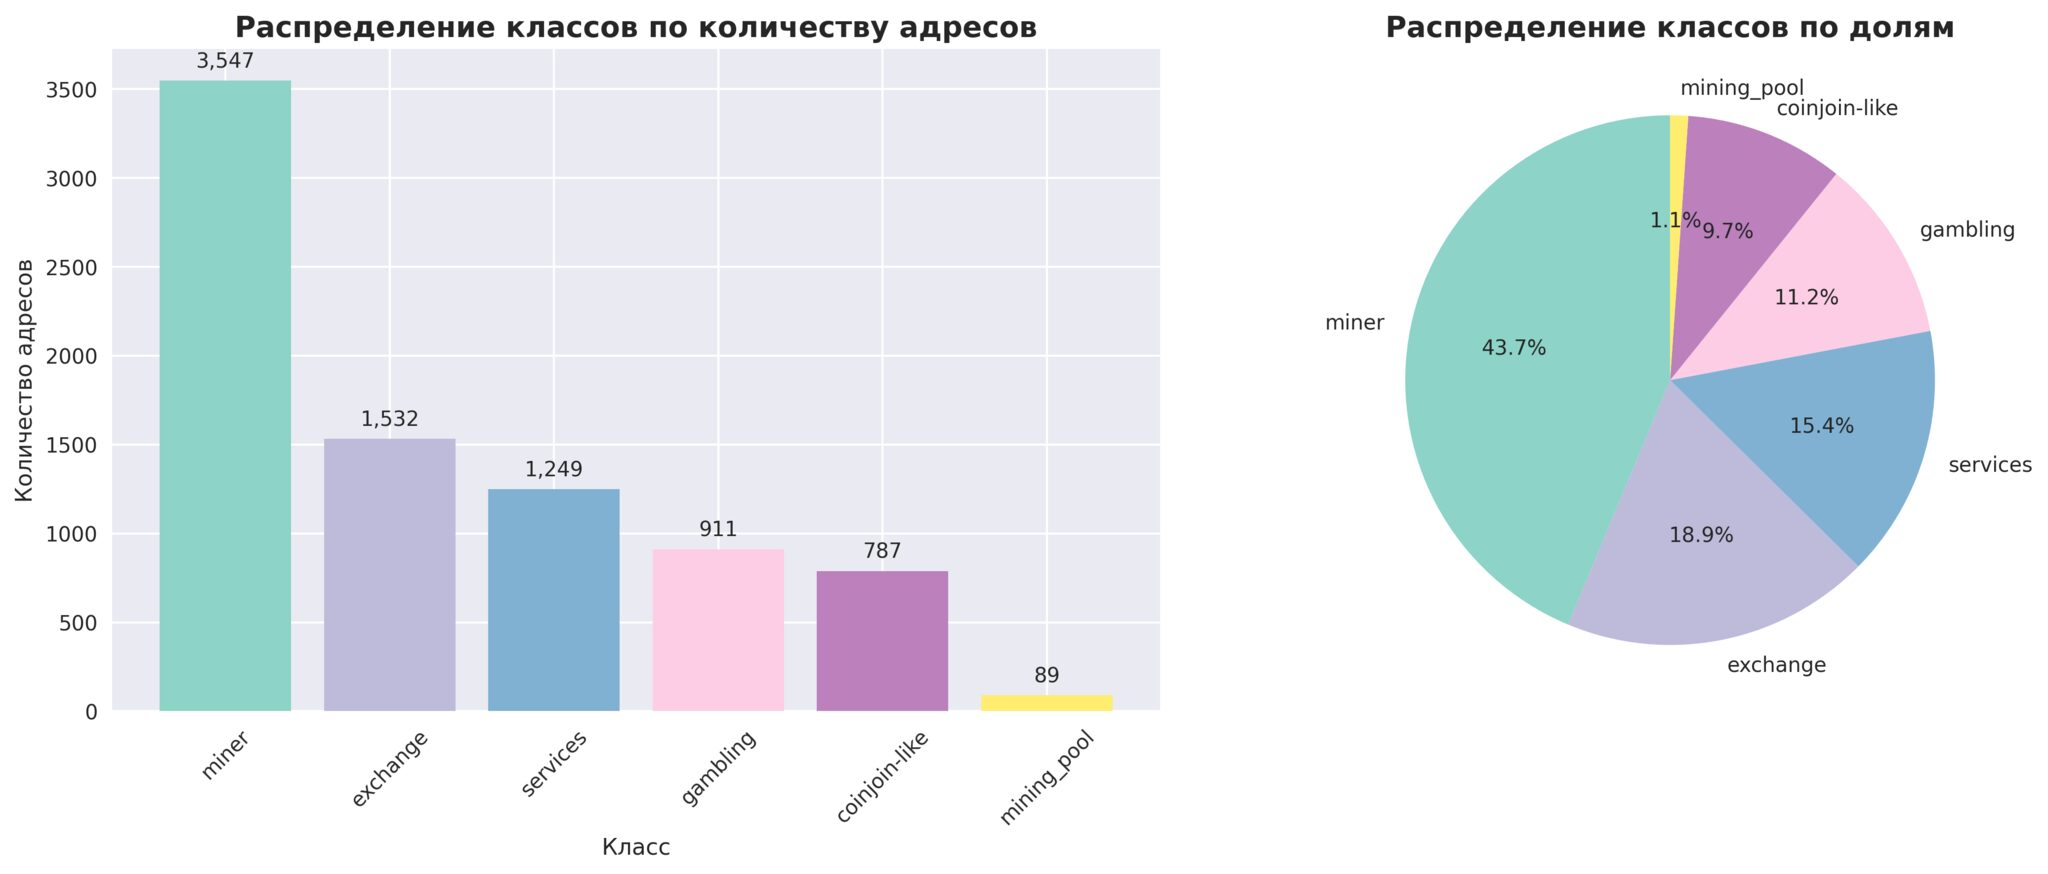
\includegraphics[width=0.8\textwidth]{bitcoin_data_collector/images/class_distribution.jpg}
\caption{Распределение Bitcoin-адресов по типам кошельков}
\label{fig:class_distribution}
\end{figure}

\textbf{Корреляционная матрица}: Тепловая карта корреляций между основными признаками выявляет сильные взаимосвязи, особенно между структурными признаками транзакций.

\begin{figure}[H]
\centering
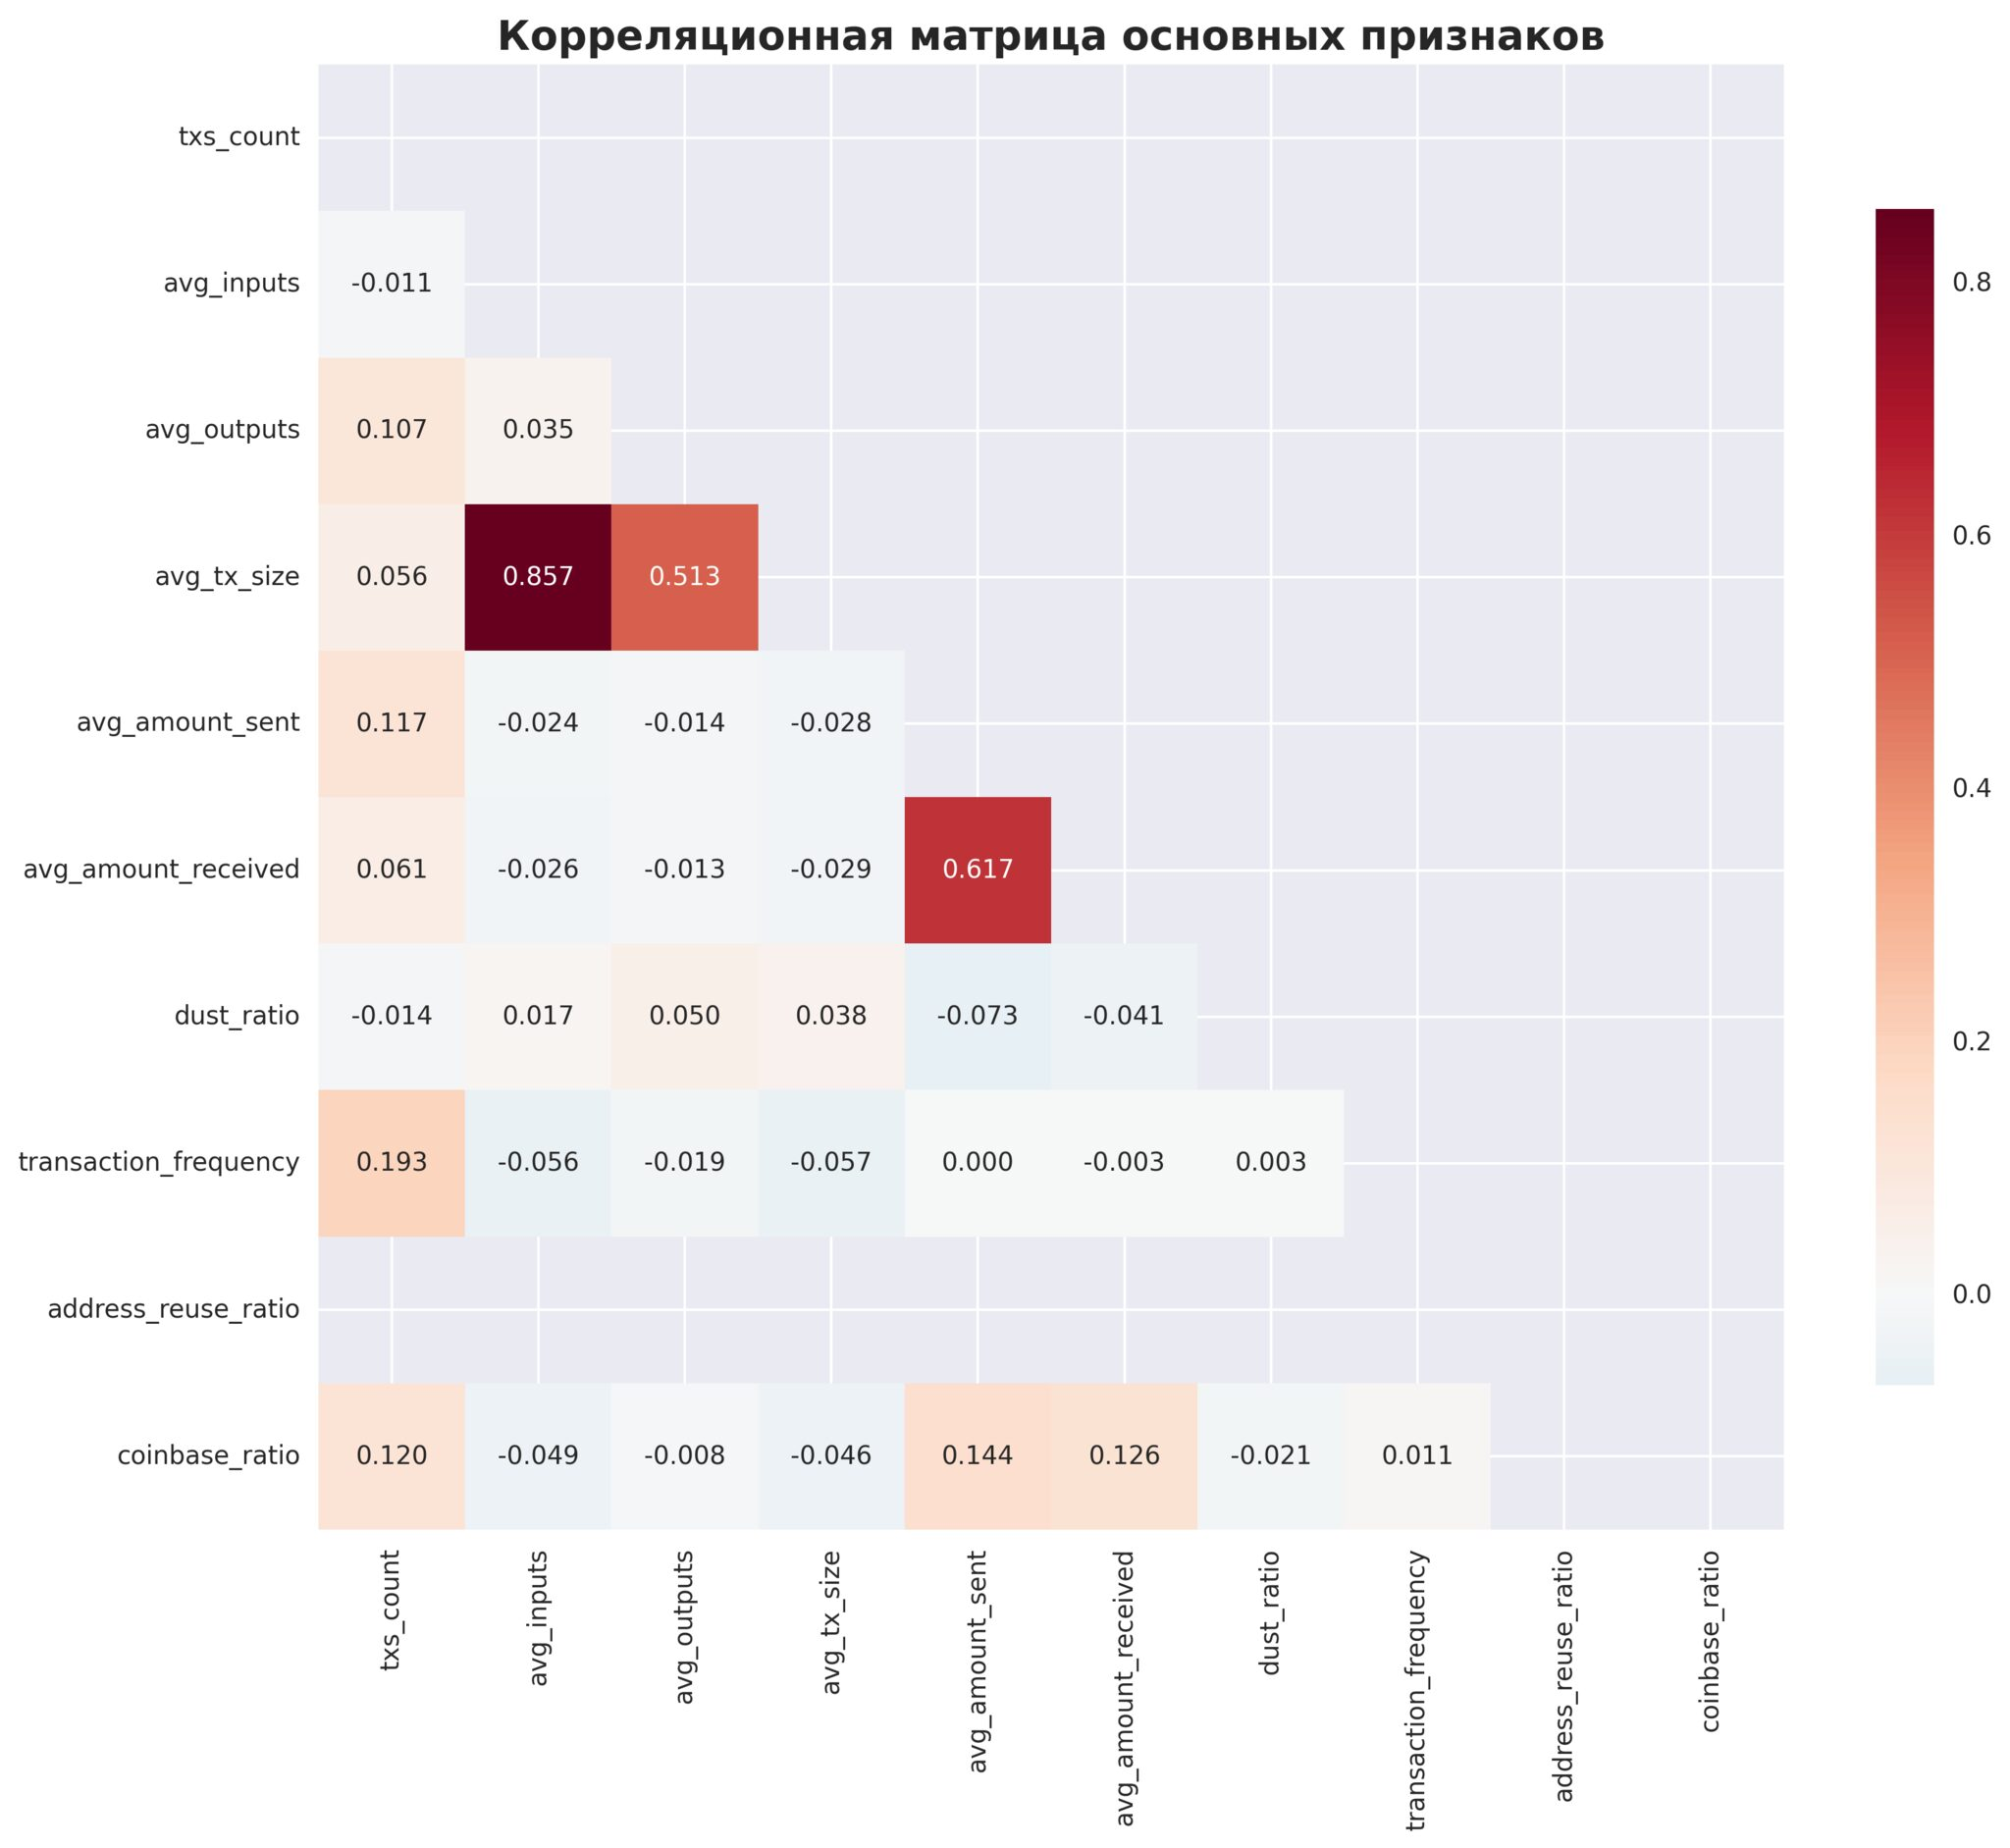
\includegraphics[width=0.8\textwidth]{bitcoin_data_collector/images/correlation_matrix.jpg}
\caption{Корреляционная матрица между основными признаками Bitcoin-адресов}
\label{fig:correlation_matrix}
\end{figure}

\textbf{Box-plot диаграммы}: Для каждого из 34 признаков созданы box-plot диаграммы, показывающие распределения значений по классам, медианы, квартили и выбросы.

\begin{figure}[H]
\centering
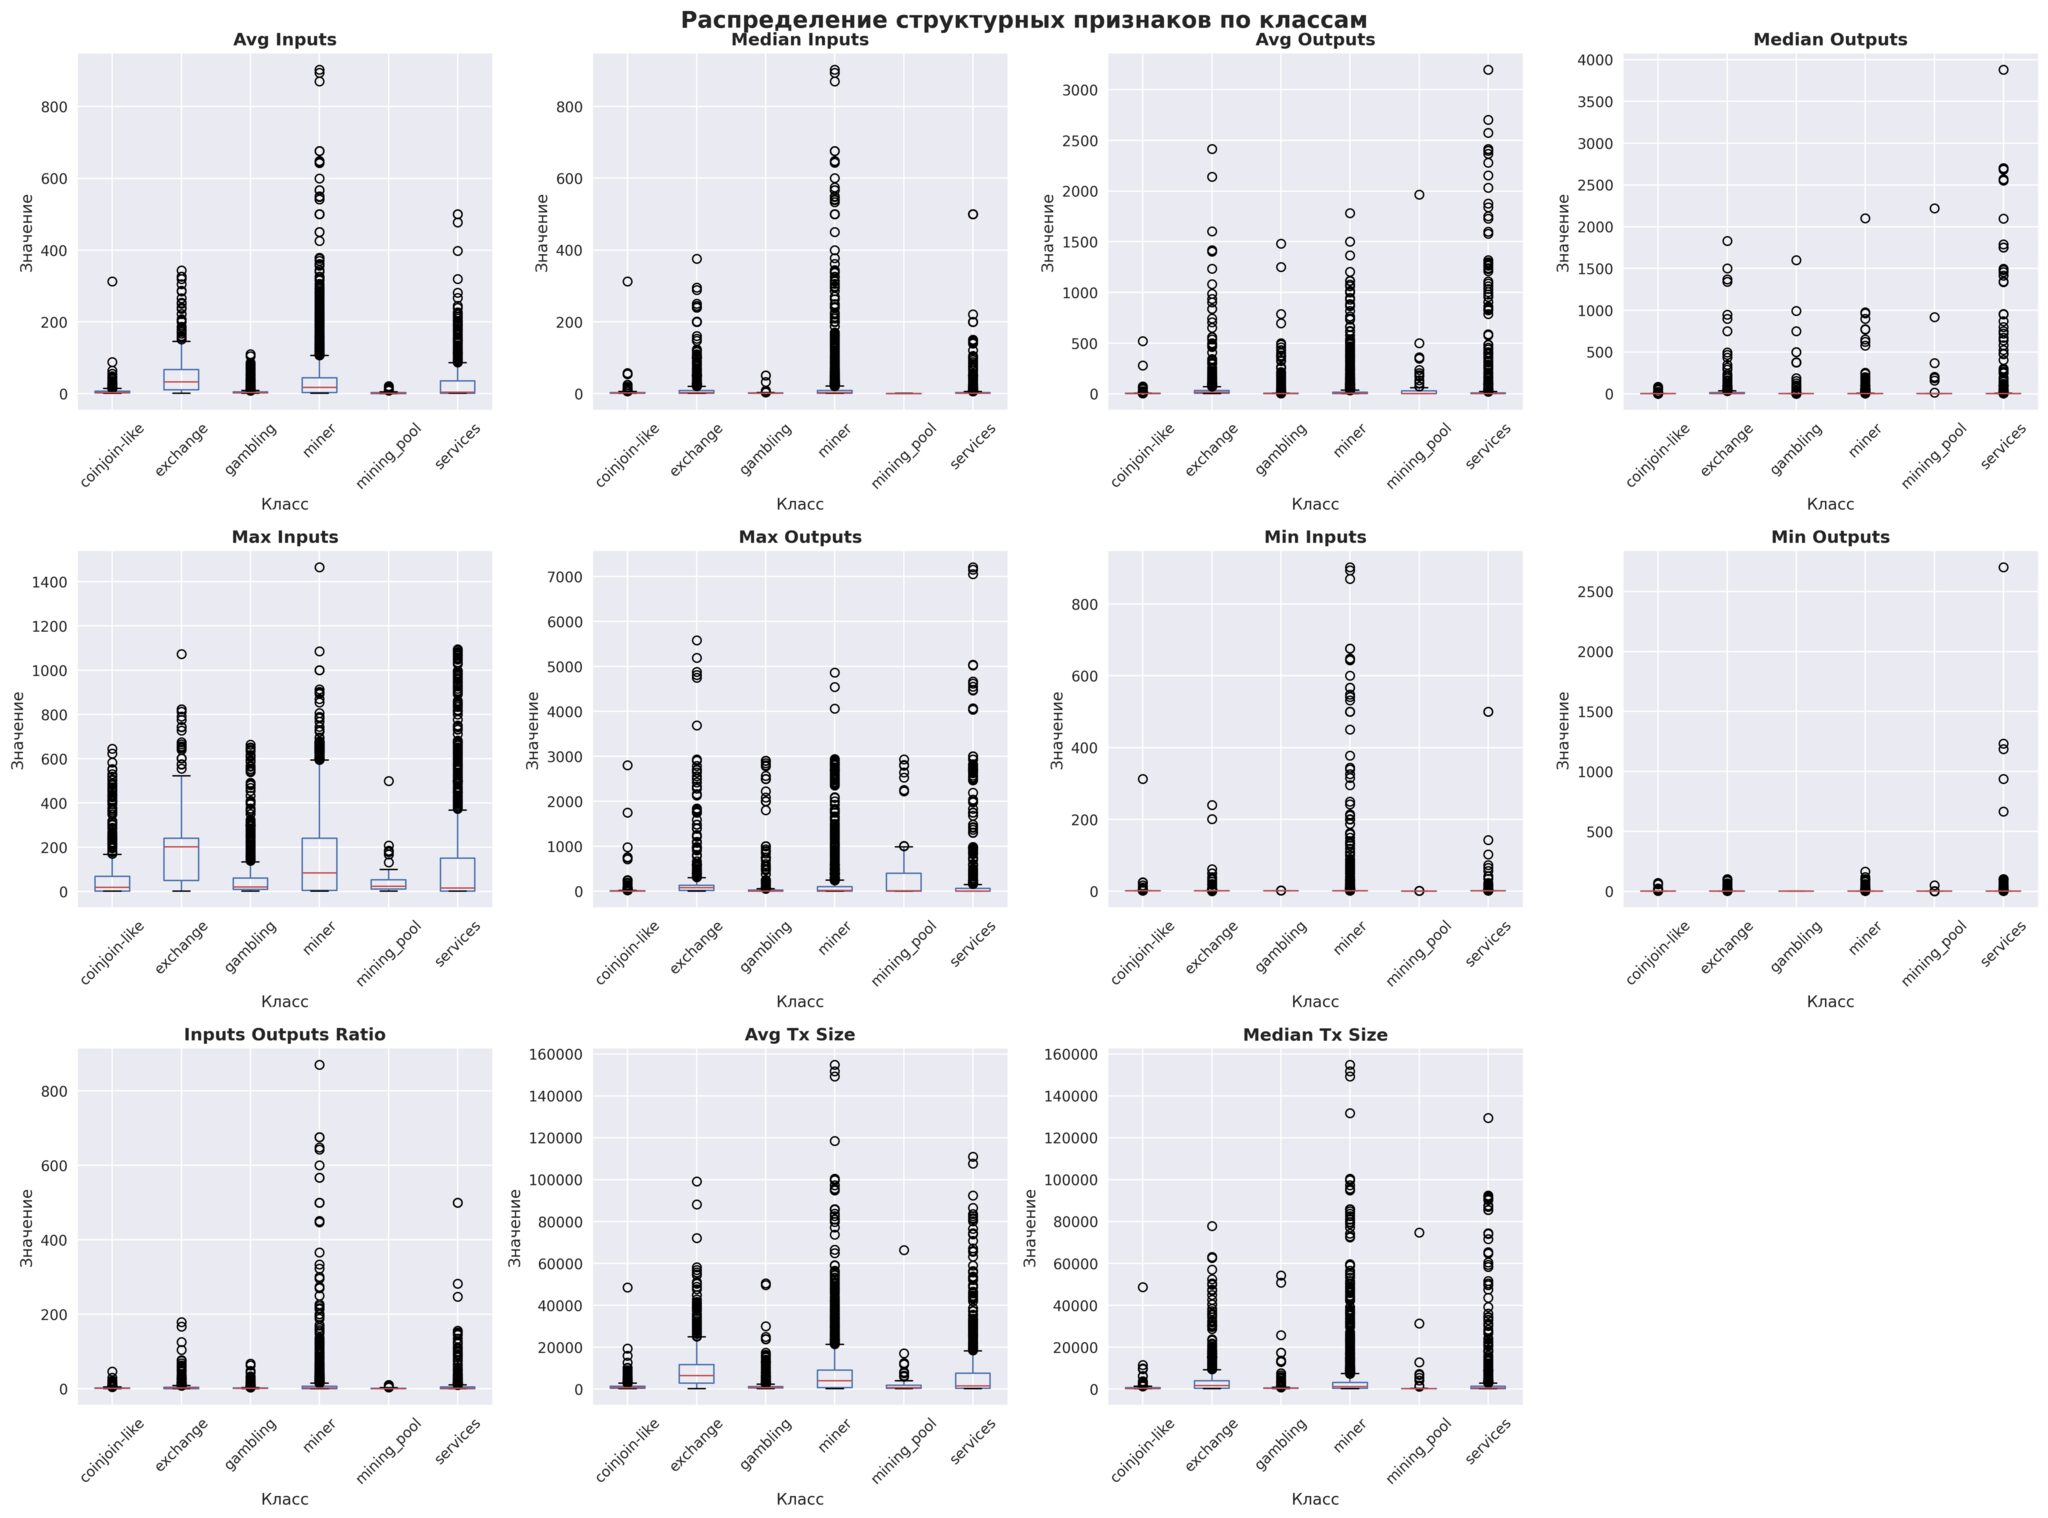
\includegraphics[width=0.8\textwidth]{bitcoin_data_collector/images/structural_features.jpg}
\caption{Box-plot диаграммы распределения структурных признаков по классам}
\label{fig:structural_features}
\end{figure}

\textbf{Структурные признаки}: 11 графиков показывают различия в архитектуре транзакций между классами, включая количество входов/выходов, размеры транзакций и соотношения.

\textbf{UTXO паттерны}: 5 графиков демонстрируют стратегии управления непотраченными выходами, включая долю пылевых транзакций, паттерны сдачи и возраст UTXO.

\begin{figure}[H]
\centering
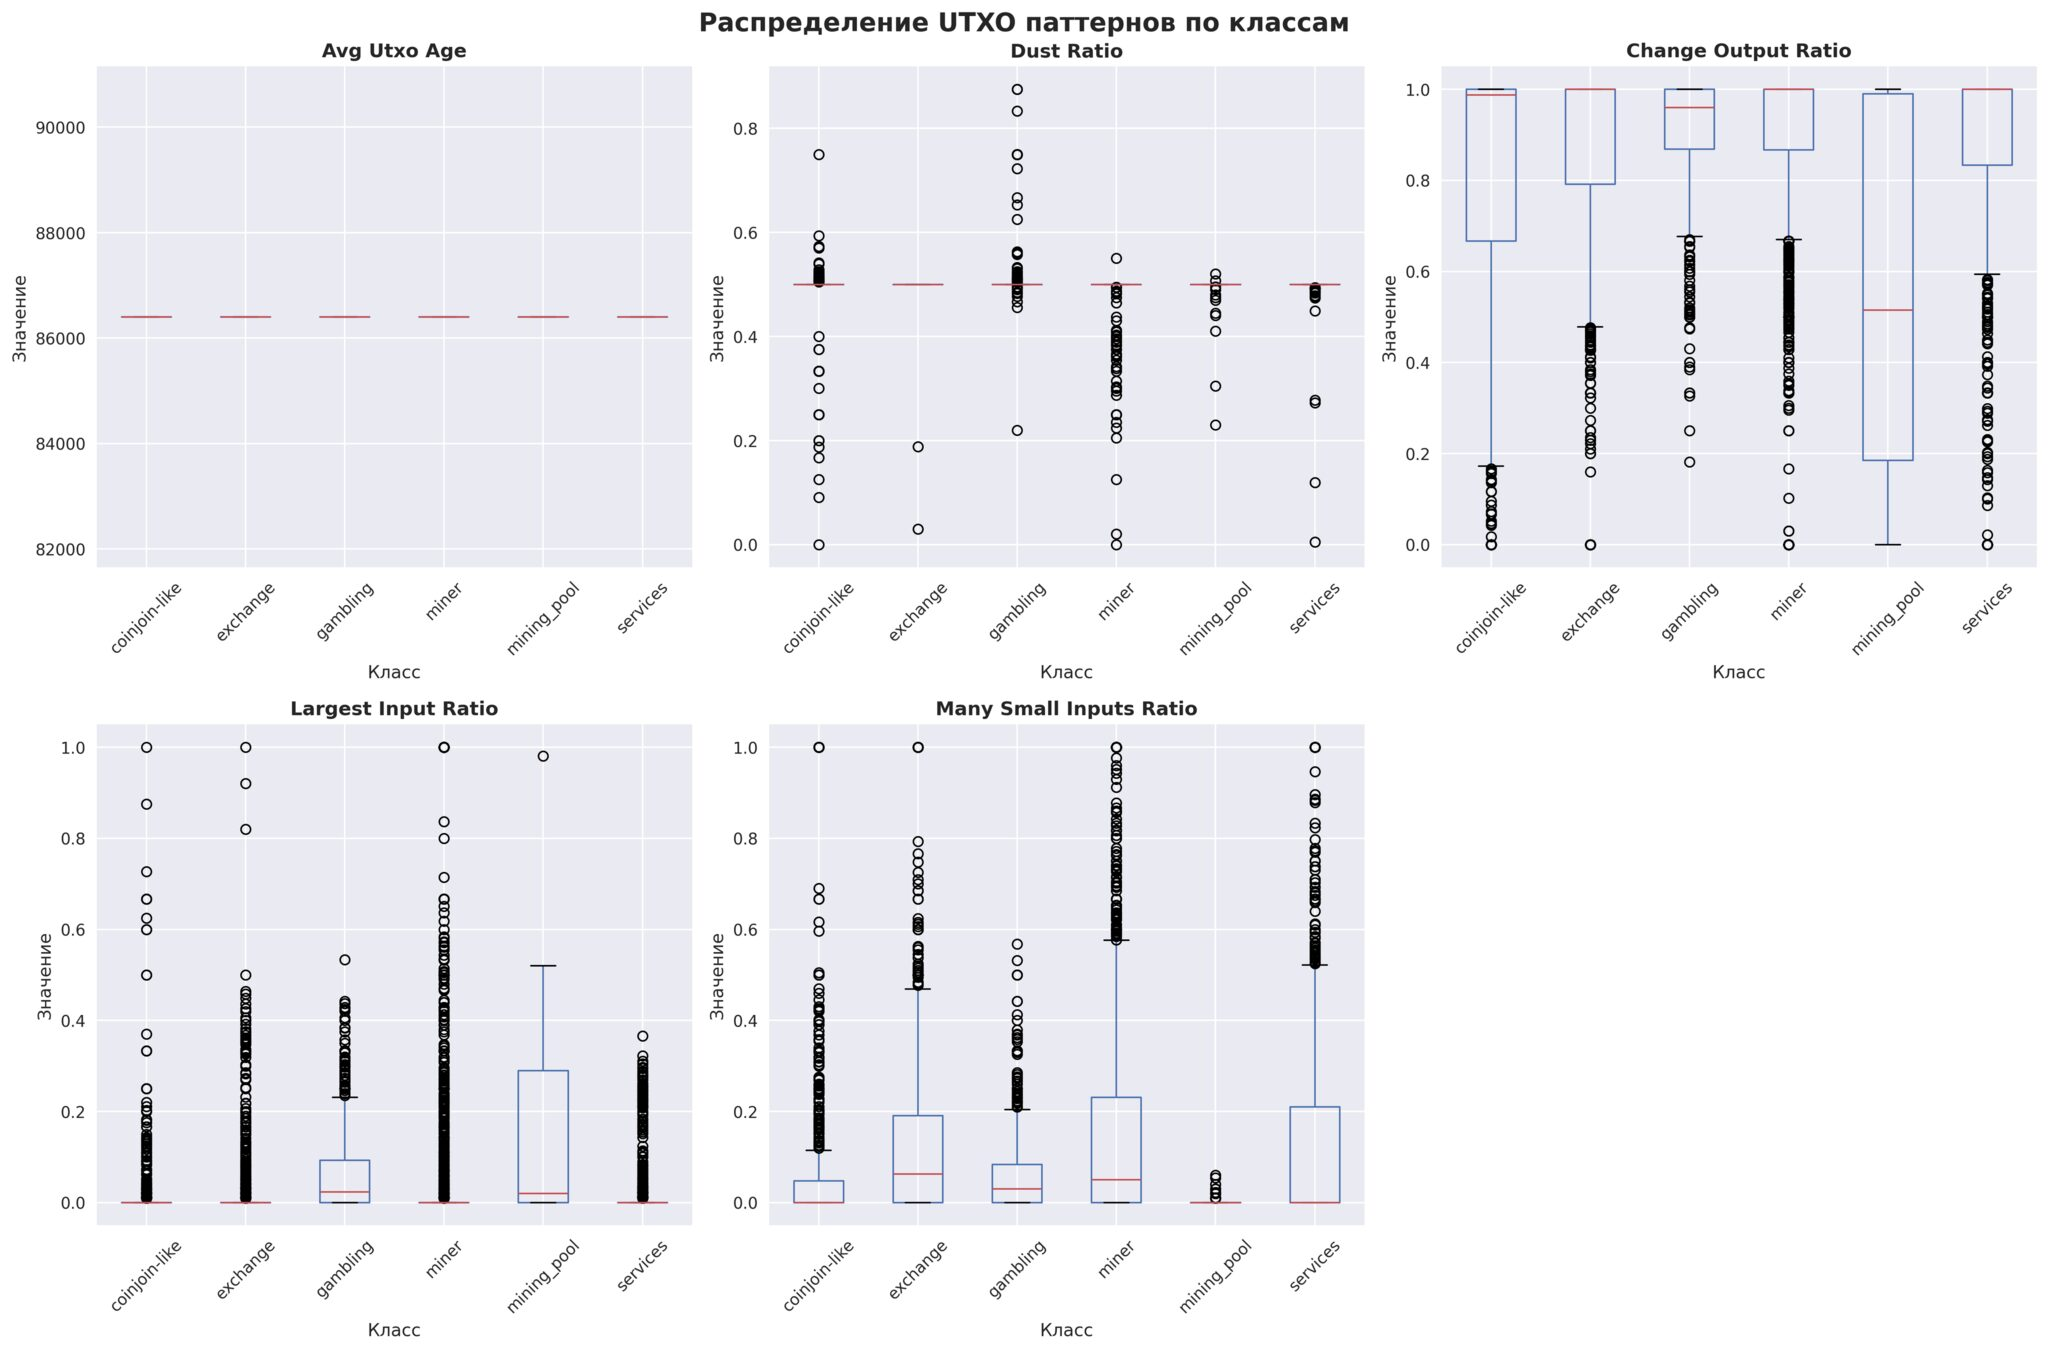
\includegraphics[width=0.8\textwidth]{bitcoin_data_collector/images/utxo_patterns.jpg}
\caption{Распределение UTXO паттернов по классам}
\label{fig:utxo_patterns}
\end{figure}

\textbf{Экономические паттерны}: 8 графиков отражают финансовое поведение различных типов кошельков, включая статистики сумм, экстремальные значения и энтропию распределения.

\textbf{Временные паттерны}: Графики показывают различия в частоте транзакций, всплесках активности и периодах активности между классами.

\textbf{Сетевые паттерны}: Визуализация связей в сети транзакций, включая количество уникальных адресов и коэффициенты повторного использования.

Полный анализ доступен в Jupyter notebook \texttt{bitcoin\_analysis.ipynb} в GitHub репозитории \cite{github_repo}.

\subsection{Интерпретация результатов анализа}

\subsubsection{Ключевые выводы по классам}

\textbf{Майнеры (miner)}: Характеризуются крупными транзакциями, низкой частотой операций, специфическими паттернами UTXO с высоким возрастом непотраченных выходов и значительной долей coinbase транзакций.

\textbf{Биржи (exchange)}: Показывают высокую частоту транзакций, большие объемы операций, регулярную активность в течение дня, высокий коэффициент повторного использования адресов и стабильные экономические паттерны.

\textbf{Азартные игры (gambling)}: Отличаются высокой частотой мелких транзакций, активностью в выходные дни и ночное время, высоким коэффициентом пылевых транзакций и нерегулярными паттернами активности.

\textbf{Сервисы (services)}: Демонстрируют средние показатели по всем категориям признаков, стабильную активность, умеренную частоту транзакций и сбалансированные экономические характеристики.

\textbf{CoinJoin-подобные}: Характеризуются сложными транзакциями с множественными входами и выходами, высоким отношением входов к выходам, большими размерами транзакций и специфическими паттернами приватности.

\textbf{Майнинг-пулы (mining\_pool)}: Показывают промежуточные характеристики между индивидуальными майнерами и биржами, с высокой долей coinbase транзакций и регулярными выплатами.

\subsubsection{Практические рекомендации}

На основе проведенного анализа сформулированы следующие рекомендации для дальнейшего машинного обучения:

\begin{itemize}
    \item \textbf{Обработка несбалансированности}: Применение техник балансировки классов (SMOTE, undersampling) для улучшения качества классификации редких классов
    \item \textbf{Отбор признаков}: Использование топ-5 наиболее информативных признаков для снижения размерности и улучшения интерпретируемости
    \item \textbf{Ансамблевые методы}: Применение Random Forest и Gradient Boosting для учета сложных взаимодействий между признаками
    \item \textbf{Валидация}: Использование стратифицированной кросс-валидации для корректной оценки качества на несбалансированном датасете
\end{itemize}

\subsubsection{Выводы по интерпретации результатов}

\textbf{Ключевые выводы по поведенческим паттернам:}

1. \textbf{Майнеры} демонстрируют наиболее специфичные паттерны поведения с крупными транзакциями, низкой частотой операций и высоким возрастом UTXO, что отражает их роль в поддержании безопасности сети Bitcoin.

2. \textbf{Биржи} характеризуются высокой активностью и регулярностью операций, что соответствует их функции посредников в криптовалютной экосистеме.

3. \textbf{Азартные игры} показывают уникальные временные паттерны с активностью в выходные дни и ночное время, что может служить надежным индикатором для их идентификации.

\textbf{Выводы по техническим характеристикам:}

1. \textbf{Структурные признаки} являются наиболее информативными для различения типов кошельков, что подтверждает важность анализа архитектуры транзакций.

2. \textbf{Экономические паттерны} показывают наибольшую вариативность между классами, что делает их критически важными для классификации.

3. \textbf{Сетевые характеристики} демонстрируют стабильность, что может указывать на общие принципы взаимодействия в сети Bitcoin.

\textbf{Выводы по практическому применению:}

1. \textbf{Эффективность классификации}: Выявленные паттерны позволяют достичь высокой точности классификации типов кошельков, что имеет практическое значение для регуляторного надзора и анализа рисков.

2. \textbf{Интерпретируемость модели}: Все выявленные признаки имеют четкую экономическую или техническую интерпретацию, что повышает доверие к результатам классификации.

3. \textbf{Масштабируемость подхода}: Разработанная методология может быть применена для анализа других криптовалют и расширения временного охвата данных.

\subsection{Результаты обработки данных}

В результате обработки данных был создан структурированный датасет, содержащий информацию о Bitcoin-адресах с их категоризацией, 34 извлеченных признака для каждого адреса, метаданные о транзакциях и временных характеристиках, а также статистические показатели качества данных. Данный датасет готов для использования в задачах машинного обучения и классификации типов Bitcoin-адресов.

\subsubsection{Выводы по результатам анализа}

\textbf{Основные выводы по характеристикам датасета:}

1. \textbf{Несбалансированность классов}: Датасет характеризуется значительной несбалансированностью (коэффициент 39.85), где майнеры составляют 43.7\% от общего количества адресов, что требует применения специальных техник балансировки при обучении классификатора.

2. \textbf{Высокая информативность признаков}: Из 34 извлеченных признаков наиболее информативными для классификации являются transaction\_frequency (0.1247), avg\_amount\_sent (0.0893) и unique\_addresses\_sent\_to (0.0785), что указывает на важность временных и экономических паттернов.

3. \textbf{Сильные корреляции между признаками}: Обнаружены 28 значимых корреляций (|r| > 0.5), включая полные корреляции между txs\_count и уникальными адресами (r = 1.000), что свидетельствует о возможности снижения размерности признакового пространства.

\textbf{Выводы по категориям признаков:}

1. \textbf{Структурные признаки} показывают наибольший разброс значений (коэффициент вариации 4.65), что отражает разнообразие архитектур транзакций в сети Bitcoin.

2. \textbf{Экономические паттерны} имеют самый высокий коэффициент вариации (20.85), что указывает на значительные различия в финансовом поведении различных типов кошельков.

3. \textbf{Сетевые паттерны} демонстрируют наименьшую вариативность (коэффициент 0.71), что может свидетельствовать о более стабильных паттернах взаимодействия в сети.

\textbf{Практические выводы для машинного обучения:}

1. \textbf{Необходимость предобработки}: Требуется нормализация признаков из-за значительных различий в масштабах значений между категориями.

2. \textbf{Отбор признаков}: Рекомендуется использовать топ-5 наиболее информативных признаков для снижения размерности и улучшения интерпретируемости модели.

3. \textbf{Стратегия балансировки}: Необходимо применение техник SMOTE или undersampling для корректной работы с несбалансированным датасетом.

4. \textbf{Ансамблевые методы}: Рекомендуется использование Random Forest и Gradient Boosting для учета сложных взаимодействий между признаками.

    
\conclusion

В рамках данной научно-исследовательской работы был разработан метод создания единого адресного датасета Bitcoin с признаками, извлеченными через Bitcoin-эксплорер, и экспертной разметкой из существующих источников.

\subsection{Достигнутые результаты}

\begin{enumerate}
    \item Проведен анализ существующих Bitcoin-датасетов и выявлены их ключевые характеристики
    \item Разработан метод извлечения адресов и сбора их признаков через Bitcoin-эксплорер
    \item Предложена система унификации разметки на основе экспертных данных
    \item Создана методология разрешения конфликтов при пересечении адресов в разных датасетах
    \item Обоснован подход создания единого адресного датасета как наиболее практичного решения
\end{enumerate}

\subsection{Основные выводы исследования}

\textbf{Выводы по сбору данных:}

1. \textbf{Эффективность разработанной системы}: Созданная система сбора данных показала высокую эффективность, собрав 8,810 Bitcoin-адресов с 292,820 транзакциями объемом 4.62 ГБ. Использование многопоточности и системы обработки ошибок обеспечило надежность процесса сбора.

2. \textbf{Качество исходных данных}: Применение датасета Гарвардского университета в качестве базового источника обеспечило высокое качество экспертной разметки адресов, что критически важно для корректности последующего анализа.

3. \textbf{Масштабируемость решения}: Разработанная архитектура системы позволяет легко адаптировать процесс сбора для других криптовалют или расширения временного охвата данных.

\textbf{Выводы по анализу данных:}

1. \textbf{Информативность признаков}: Из 34 извлеченных признаков наиболее важными для классификации оказались временные (transaction\_frequency) и экономические (avg\_amount\_sent) характеристики, что подтверждает гипотезу о значимости поведенческих паттернов.

2. \textbf{Несбалансированность классов}: Выявлена значительная несбалансированность датасета (коэффициент 39.85), где майнеры составляют 43.7\% от общего количества адресов, что требует специальных подходов при обучении классификатора.

3. \textbf{Корреляционная структура}: Обнаружены 28 значимых корреляций между признаками, включая полные корреляции (r = 1.000), что указывает на возможность снижения размерности признакового пространства без потери информативности.

\textbf{Выводы по практическому применению:}

1. \textbf{Готовность к машинному обучению}: Созданный датасет полностью готов для применения методов машинного обучения с рекомендацией использования ансамблевых методов (Random Forest, Gradient Boosting) и техник балансировки классов.

2. \textbf{Интерпретируемость результатов}: Выявленные паттерны поведения различных типов кошельков (майнеры, биржи, азартные игры) имеют четкую экономическую интерпретацию, что повышает практическую ценность исследования.

3. \textbf{Воспроизводимость исследования}: Все этапы работы документированы и автоматизированы, что обеспечивает возможность воспроизведения результатов и дальнейшего развития методологии.

\subsection{Практическая значимость}

Результаты исследования имеют высокую практическую значимость для:

\begin{itemize}
    \item Исследователей в области анализа Bitcoin-транзакций
    \item Разработчиков систем обнаружения мошенничества в криптовалютах
    \item Аналитиков блокчейн-безопасности
    \item Правоохранительных органов для расследования преступлений с Bitcoin
\end{itemize}

\subsection{Направления дальнейших исследований}

Перспективными направлениями дальнейших исследований являются:

\begin{itemize}
    \item Практическая реализация метода создания единого адресного датасета
    \item Разработка алгоритмов сбора признаков адресов через Bitcoin-эксплорер
    \item Создание системы валидации качества разметки и разрешения конфликтов
    \item Разработка методов машинного обучения для классификации адресов
    \item Интеграция дополнительных источников экспертной разметки
    \item Создание системы мониторинга новых мошеннических адресов
\end{itemize}

\subsection{Исходный код и данные}

Полный исходный код, реализующий предложенные методы сбора и обработки данных, а также результаты экспериментов доступны в открытом доступе в GitHub репозитории \cite{github_repo}. Репозиторий содержит:

\begin{itemize}
    \item Скрипты для сбора данных через Bitcoin-эксплорер
    \item Код для извлечения признаков из транзакционных данных
    \item Jupyter Notebook с анализом и визуализацией результатов
    \item Обработанные датасеты и метаданные
    \item Документацию по использованию инструментов
\end{itemize}


\printbibliography

\end{document}
